%=====================================================
% Specify the document type (book, article)
%=====================================================

\newcommand{\doctype}{book}							% book or article

%=====================================================
% Specify part names (only for books)
%=====================================================

\newcommand\parta{Audit Report}


%=====================================================
% Specify which lists you want
%=====================================================

\newcommand\listofs{true}									% Any ``ListOfs?''
\newcommand\toc{true}										% Table of Contents
\newcommand\lot{true}										% List of Tables
\newcommand\lof{true}										% List of Figures
\newcommand\loe{true}										% List of Exhibits
\newcommand\lod{true}										% Include Distribution List

%=====================================================
% Load the main layout file
%=====================================================

%-----------------------------------------------------
% Overall Geometry of the Document
%-----------------------------------------------------
\documentclass[12pt,a4paper,fleqn,twoside]{article}	  	
\usepackage{cmap}

\usepackage[hmarginratio=1:1]{geometry}
\geometry{%
  left=2.5cm,				% left margin
  top=3.5cm,				% top  margin
  textwidth=16cm,		% width of text block
  textheight=21.0cm}	% height of text block
\setlength{\headheight}{1cm}					    % height of header
\setlength{\headsep}{1cm}							% distance of header
\setlength{\footskip}{1.5cm}					    % distance of footer
\renewcommand{\baselinestretch}{1.0}     % 1line distance

%----------------------------------------------------- 
% Language
%-----------------------------------------------------
\usepackage[english]{varioref}			  
\usepackage[american]{babel}
\usepackage[utf8]{inputenc}
\usepackage[T1]{fontenc}
\usepackage{csquotes}  
\selectlanguage{american}


%-----------------------------------------------------
% Headers
%-----------------------------------------------------
\usepackage{fancyhdr}
\usepackage[Sonny]{sty/fncychap/fncychap}
\ChNumVar{\fontsize{60}{62}}


%-----------------------------------------------------
% Floats, Tables, Equations
%-----------------------------------------------------
\usepackage[hang]{caption} 
\usepackage[section] {placeins}
\usepackage{float}
\usepackage{colortbl}
\usepackage{booktabs}
\usepackage{latexsym}
\setcounter{totalnumber}{4}                     % max. no. of floats / page
\setcounter{topnumber}{2}                       % max. no. of floats / page top
\setcounter{bottomnumber}{2}                 % max. no. of floats / page bottom
\renewcommand{\topfraction}{1}           % half the page can be filled with
\renewcommand{\bottomfraction}{1}    % floats for top and bottom half
\usepackage{wrapfig}

%-----------------------------------------------------
% Listings
%-----------------------------------------------------
\usepackage{listings}
\definecolor{lstemph}{rgb}{0,0.39,0} 
\definecolor{lstnumbers}{rgb}{0.59,0.57,0.43} 
\definecolor{lstcomments}{rgb}{0.33,0.35,0.69} 
\lstloadlanguages{Java,C++}
\lstset{language=Java,
		extendedchars=true,
        basicstyle=\ttfamily\tiny,
        keywordstyle=\color{lstnumbers},
        identifierstyle=\color{black}, 
        commentstyle=\color{lstcomments},
        stringstyle=\ttfamily\color{blue},
        showstringspaces=true,
        numbers=left,
        stepnumber=1,
        numberstyle=\tiny\ttfamily\color{lstnumbers},
        numbersep=12pt,
        frame=single,
        fontadjust=true,
        xleftmargin=3.5pt,
        xrightmargin=3.5pt,
        escapeinside={(*}{*)}}

%-----------------------------------------------------
% Processing of the document
%-----------------------------------------------------
% Includex is for combining documents.
% It is obsolete and throws warnings,
% so we do not use it as long as we do not
% need it. See:
%
% http://www.tex.ac.uk/cgi-bin/texfaq2html?label=multidoc
% 
%\usepackage{sty/includex/includex}

%-----------------------------------------------------
% Hyperref
%-----------------------------------------------------
%\ifx\pdfoutput\undefined
%\usepackage[ps2pdf]{hyperref}
%\else
\usepackage[%pdftex,
            pdfpagemode={UseOutlines},
            pdfstartview={FitH},
            colorlinks=true,   
            linkcolor={blue},
            citecolor={blue}, 
            urlcolor={blue},
            bookmarks=true,
            bookmarksopen=true,
            %pdfpagemode=FullScreen,
            plainpages=false,
            pdfpagelabels]{hyperref} 

%-----------------------------------------------------
% Nomenclature / Glossary
%-----------------------------------------------------

%\usepackage[
%  style=altlist,
%  hypertoc=true,
%   hyper=true,
%   number=none,
%   hyperacronym=true,
%   acronym=true %dieser Parameter ist der wichtige
% ]{sty/glossary/glossary}
% \setacronymnamefmt{\gloshort}
% \makeglossary
% \makeacronym

\usepackage[
nonumberlist, %do not show page numbers
acronym,        %generate acronym listing
toc,                %show listings as entries in table of contents
section]         %use section level for toc entries
{glossaries}

%
% Patch Glossaries so that only the first occurrence of a given glossary entry
% is converted to a hyperlink, in order to avoid cluttering.
%
\makeatletter
%% patch first occurence of "\@gls@link[#1]{#2}{\@glo@text}", as this is the one for \glsused{#2}
\patchcmd{\@gls@}
  {\@gls@link[#1]{#2}{\@glo@text}}
  {\@gls@link[#1,hyper=false]{#2}{\@glo@text}}
  {}{}
\patchcmd{\@glspl@}
  {\@glspl@link[#1]{#2}{\@glo@text}}
  {\@glspl@link[#1,hyper=false]{#2}{\@glo@text}}
  {}{}
\patchcmd{\@Gls@}
  {\@gls@link[#1]{#2}}
  {\@gls@link[#1,hyper=false]{#2}}
  {}{}
\patchcmd{\@GLS@}
  {\@gls@link[#1]{#2}{\MakeUppercase{\@glo@text}}}
  {\@gls@link[#1,hyper=false]{#2}{\MakeUppercase{\@glo@text}}}
  {}{}  
\makeatother

%
% Generate a list of symbols
%
\newglossary[slg]{symbolslist}{syi}{syg}{List of Symbols}

%
% Make sure first character of glossary entry name is uppercase
%
\renewcommand{\glsnamefont}[1]{\makefirstuc{#1}}

%
% Remove the dot at the end of glossary descriptions
%
\renewcommand*{\glspostdescription}{}

%
% Activate glossary commands
%
\makeglossaries

%
% Load the glossary definitions the user writes
%
%=====================================================
% Acronyms
%=====================================================

%-----------------------------------------------------
% Samples
%-----------------------------------------------------

% Usage:
% \gls{AD} is pretty interesting. If we do reference a glossary entry,
% like, \gls{glos:AD}, that one of course has to be defined over there.

% An acronym with a glossary entry not hyperlinked
% \newacronym{AD}{AD}{Active Directory\protect\glsadd{glos:AD}}

% Geek Version, with hyperlink to glossary
% \newglossaryentry{AD}{
%   type=\acronymtype,
%   name=AD,
%   first=Active Directory (AD),
%   firstplural={Active Directories (AD's)},
%   description=\glslink{glos:AD}{Active Directory}
% }

%----------------------------------------------------- 
% Content
%-----------------------------------------------------

%<content>%



%</content>%


%-----------------------------------------------------
% Default Content
%-----------------------------------------------------

    
 
   
 
 
 
  
  








































%=====================================================
% Symbols
%=====================================================

%-----------------------------------------------------
% Samples
%-----------------------------------------------------

% Usage:
% \section{Some Greek symbols}
% If you calculate with \gls{symb:Pi} you always get an irrational result, because 
% \gls{symb:Pi} itself is irrational. As a matter of fact, there are \gls{symb:Phi} 
% and \gls{symb:Lambda}, too.

%Some entries for the list of symbols
\newglossaryentry{symb:Pi}{
  type=symbolslist,
  name=$\pi$,
  description={A mathematical constant whose value is the ratio of any circle's circumference to its diameter.},
  sort=symbolpi
}
\newglossaryentry{symb:Phi}{
  type=symbolslist,
  name=$\varphi$,
  description={An angle.},
  sort=symbolphi
}
\newglossaryentry{symb:Lambda}{
  type=symbolslist,
  name=$\lambda$,
  description={Lambda indictes an eigenvalue in the mathematics  of linear algebra.},
  sort=symbollambda
}

%-----------------------------------------------------
% Content
%-----------------------------------------------------

%<content>%



%</content>%



























%=====================================================
% Glossary
%=====================================================

%-----------------------------------------------------
% Samples
%-----------------------------------------------------

% Usage:
% \gls{glos:AD} is pretty interesting. If we have a cross reference from
% the acronyms, we can also directly go to that using \gls{AD}; this
% requires then that over there, we have something like
%  see=[Glossary:]{\gls{glos:AD}}, 
%  description=\glslink{glos:AD}{Active Directory}

% \newglossaryentry{glos:AD}{
% name=Active Directory,
% description={Active Directory is the directory service for 
% Windows based networks, that allows central organization and 
% administration of any network resource.
% It allows a single-sign-on concept independent from network 
% topologies or network protocols. As a prerequisite you need 
% a Windows Server acting as Domain Controller. This computer 
% stores all necessary data, e.\,g.~usernames and corresponding 
% passwords.}
% }


%-----------------------------------------------------
% Content
%-----------------------------------------------------

%<content>%



%</content>%















%
% These commands actually create / update the different
% indices / glossaries
%
%makeindex -s document.ist -t document.alg -o document.acr document.acn
%makeindex -s document.ist -t document.glg -o document.gls document.glo
%makeindex -s document.ist -t document.slg -o document.syi document.syg
%makeindex document

%-----------------------------------------------------
% Index
%-----------------------------------------------------

\usepackage{makeidx}

%-----------------------------------------------------
% Media
%-----------------------------------------------------

%\renewcommand{\video}[6]{% file xpos ypos width height controls
%  \vspace{#3}\hspace{#2}{\pdfannot width #4 height #5 depth 0cm {%
%   /Subtype /Movie  
%   /Movie  << /F (#1) >> 
%   /A << /ShowControls #6 /Rate 1 >>
%   }}}
%\fi

\usepackage{sty/easymovie/easymovie}


%-----------------------------------------------------
% Equations
%-----------------------------------------------------

\usepackage{amssymb,amsmath}

%
% Label only referened equations
%
%\usepackage{autonum}

%
% Default to roman style
%
%\everymath{\rm}





%-----------------------------------------------------
% Font Settings
%-----------------------------------------------------
\renewcommand*\captionlabelfont{\bfseries}	
\renewcommand*\captionsize{\itshape}		

\makeatletter
\renewcommand{\section}{\@startsection{section}{1}{\z@}%
    {-2.2ex \@plus-1ex \@minus -.2ex}{1.3ex \@plus.2ex}%
    {\reset@font\large\bfseries}}
\renewcommand{\subsection}{\@startsection{subsection}{2}{\z@}%
    {-1.5ex \@plus -1ex \@minus-.2ex}{0.8ex \@plus.2ex}%
    {\reset@font\normalsize\bfseries}}
\renewcommand{\subsubsection}{\@startsection{subsubsection}{3}{\z@}%
     {-1.2ex\@plus -1ex \@minus -.2ex}{0.5ex \@plus .2ex}%
     {\reset@font\normalsize}}
 \renewcommand{\paragraph}{\@startsection{paragraph}{4}{0mm}%
  {1ex \@plus1ex \@minus.2ex}%
  {-1em}%
  {\normalfont\normalsize\it}}
 \renewcommand{\subparagraph}{\@startsection{subparagraph}{5}{\parindent}%
  {2.0ex \@plus1ex \@minus .2ex}%
  {-1em}%
  {\normalfont\normalsize\it}}     
\makeatother

%-----------------------------------------------------
% Itemizes etc.
%-----------------------------------------------------
\renewcommand{\labelitemi}{$\triangleright$}
\renewcommand*\descriptionlabel[1]{\hspace\labelsep
                                \normalfont\itshape #1}

%-----------------------------------------------------
% Widow etc. compensations
%-----------------------------------------------------
\clubpenalty10000					
\widowpenalty10000					
\hbadness 10000
\scrollmode
\sloppy


%-----------------------------------------------------
% Depth of Table of Contents
%-----------------------------------------------------
\setcounter{secnumdepth}{10}				
\setcounter{tocdepth}{3}

%-----------------------------------------------------
% PDF or not
%-----------------------------------------------------
\usepackage{ifpdf}


%-----------------------------------------------------
% Footnotes
%-----------------------------------------------------
\usepackage[flushmargin, hang]{footmisc}		
\usepackage{sty/botfnote/botfnote}
%\usepackage{endnotes}
\usepackage[backref]{sty/enotez/enotez}

%Disable to have actual footnotes
%\let\footnote=\endnote
%\let\footnotemark=\endnotemark
%\let\footnotetext=\endnotetext
 %remember to substitute \value{footnote} by \endnote or vice versa
 
\ifpdf
  \usepackage{sty/hyperendnote/hyperendnote}  
\fi

%\renewcommand\enoteformat{\noindent
%\setlength\parindent{12pt}\makebox[0pt][r]{\hyperlink{Hendnotepage.\theenmark}{%
% \hbox{$^{\theenmark}$}}\,}}
%\renewcommand\enotesize{\scriptsize}

%\renewcommand\enoteformat{\noindent
%\leftskip=-2.5em \makebox[2.5em][r]{\theenmark.\ }\hangindent 2.5em}


%-----------------------------------------------------
% Graphics
%-----------------------------------------------------
\usepackage{graphicx}
\ifpdf
  \graphicspath{{pdf/}}
  \pdfcompresslevel=9
  \DeclareGraphicsExtensions{.pdf}
  \DeclareGraphicsRule{.pdf}{pdf}{.pdf}{}
\else
  \graphicspath{{eps/}}
  \DeclareGraphicsExtensions{.eps}
  \DeclareGraphicsRule{.eps}{eps}{.eps}{}
\fi

%\ifx\pdfoutput\undefined
%\usepackage[dvips]{graphicx}
% \graphicspath{{eps/}}
% \DeclareGraphicsExtensions{.eps}
% \DeclareGraphicsRule{.eps}{eps}{.eps}{}
% \else
% \usepackage[pdftex]{graphicx} 
% \graphicspath{{pdf/}}
% \pdfcompresslevel=9
% \DeclareGraphicsExtensions{.pdf}
% \DeclareGraphicsRule{.pdf}{pdf}{.pdf}{}
% \fi

\usepackage{color}
\usepackage{array}

%-----------------------------------------------------
% Makros
%-----------------------------------------------------
%=====================================================
% Makros
%=====================================================

%-----------------------------------------------------
% Simple Substitutions:
%-----------------------------------------------------

\def\ni{\noindent}
\def\usw{$[\dots]$}
\def\daher{$\rightarrow$}
\def\tab{\hspace{2 cm}}
\def\fn{\footnote}
\def\en{\endnote}
\def\Unterschrift{\newline \includegraphics[width=4cm]{unter} \newline}
\def\unterschrift{\Unterschrift}
\newcommand{\bs}{$\backslash$}
 \def\LRA{\Leftrightarrow\mkern40mu}
 \def\RA{\Rightarrow\mkern40mu}
 
%-----------------------------------------------------
% dangerous / ddangerous etc. environments a la Knuth: 
%-----------------------------------------------------

\font\manual=manfnt
\def\dbend{{\manual\char127}}
\def\d@nger{\medbreak\begingroup\clubpenalty=10000
  \def\par{\endgraf\endgroup\medbreak}  
\noindent\hang\hangafter=-2  \hbox 
to0pt{\hskip-\hangindent\dbend\hfill}\ninepoint}
\outer\def\danger{\d@nger}
\def\dd@nger{\medbreak\begingroup\clubpenalty=10000
  \def\par{\endgraf\endgroup\medbreak} 
\noindent\hang\hangafter=-2  \hbox 
to0pt{\hskip-
\hangindent\dbend\kern1pt\dbend\hfill}\ninepoint} 
\outer\def\ddanger{\dd@nger}
\def\enddanger{\endgraf\endgroup}

\newsavebox{\fmbox}
\newenvironment{notdangerous}
{
 \begin{lrbox}{\fmbox}
 \begin{minipage}[t]{1cm}~\end{minipage}
 \begin{minipage}[t]{1.5cm}\hspace{\fill}~\end{minipage}
 \begin{minipage}[t]{0.1cm}~\end{minipage}
 \begin{minipage}[t]{12.5cm}
}
{\end{minipage}\end{lrbox}\usebox{\fmbox}
}
\newenvironment{dangerous}
{
 \begin{lrbox}{\fmbox}
 \begin{minipage}[t]{0.2cm}~\end{minipage}
 \begin{minipage}[t]{1.5cm}\hspace{\fill}\dbend\end{minipage}
 \begin{minipage}[t]{0.1cm}~\end{minipage}
 \begin{minipage}[t]{10.8cm}
}
{\end{minipage}\end{lrbox}\usebox{\fmbox}
}
\newenvironment{ddangerous}
{
 \begin{lrbox}{\fmbox}
 \begin{minipage}[t]{0.2cm}~\end{minipage}
 \begin{minipage}[t]{1.5cm}\hspace{\fill}\dbend\dbend\end{minipage}
 \begin{minipage}[t]{0.1cm}~\end{minipage}
 \begin{minipage}[t]{10.8cm}
}
{\end{minipage}\end{lrbox}\usebox{\fmbox}
}
\newenvironment{dddangerous}
{
 \begin{lrbox}{\fmbox}
 \begin{minipage}[t]{0.2cm}~\end{minipage}
 \begin{minipage}[t]{1.5cm}\hspace{\fill}\dbend\dbend\dbend\end{minipage}
 \begin{minipage}[t]{0.1cm}~\end{minipage}
 \begin{minipage}[t]{10.8cm}
}
{\end{minipage}\end{lrbox}\usebox{\fmbox}
}

%-----------------------------------------------------
% Other environments:
%-----------------------------------------------------

\newcommand{\companyfooter} {
\vspace*{0.2cm}
\setlength{\tabcolsep}{0.05cm}
\tiny
\centerline{
\begin{tabular}{p{1.5cm}p{4.5cm}p{6.0cm}p{0.5cm}p{2.96cm}}
\toprule[0.25pt]
\makebox[1.50cm][l]{Module:} &
\makebox[4.50cm][l]{\mnbook}&
\makebox[6.00cm][c]{\mnname}&
\makebox[0.50cm][l]{$\:$Date:}&
\makebox[2.96cm][r]{\today}
\\%\midrule[0.15pt]
\makebox[1.50cm][l]{Document:} &
\makebox[4.50cm][l]{\mnsubtitle}&
\makebox[6.00cm][c]{\mnsubsubtitle\ (\mnmoduleweek)}&
\makebox[0.50cm][l]{$\:$Version:}&
\makebox[2.96cm][r]{\mnversion}
\\
\bottomrule[0.25pt]
\end {tabular}
}}



%=====================================================
% Configuration of the Bibliography.
%
% Has to be in the main document because of a limitation of TeXlipse
%
% http://sourceforge.net/projects/texlipse/forums/forum/451977/topic/4614646
%=====================================================
 
\usepackage[style=apa,citestyle=authoryear,backend=biber,maxnames=3,minnames=1,sorting=nyt,sortcites=true,block=space,safeinputenc,natbib=true,backref=true,uniquename=init]{biblatex}
\DeclareLanguageMapping{american}{american-apa}
\addbibresource{Bibliography.bib}  


% \DeclareLanguageMapping{english}{english-apa}
%\usepackage{biblatex-science}

%\DeclareBibliographyDriver{online}{%
 % \usebibmacro{bibindex}%
 % \usebibmacro{begentry}%
  %\ifnameundef{author}
  %  {\iflistundef{organization}
   %   {\BibliographyWarning{No author nor organisation on Online entry}}
    %  {\printlist{organization}}}
  %  {\usebibmacro{author/editor+others/translator+others}}
  %\setunit{\labelnamepunct}
 % \newblock
 % \usebibmacro{title}%
  %\setunit{}%\newunit
  %\printlist{language}%
  %\printfield{note}%
  %\newunit\newblock
  %\setunit{\bibpagerefpunct}\newblock
  %\usebibmacro{pageref}%
  %\usebibmacro{finentry}}



%\DeclareLanguageMapping{english}{custom-english-ordinal-sscript} 
%\DeclareFieldFormat{edition}{\ifinteger{#1}{\mkbibordedition{#1}\addthinspace{}ed.}{#1\isdot}}
%\renewcommand{\labelnamepunct}{\addcolon\addspace}
%\renewcommand{\mkbibnamefirst}[1]{\textsc{#1}}
%\renewcommand{\mkbibnamelast}[1]{\textsc{#1}}
%\renewcommand{\mkbibnameprefix}[1]{\textsc{#1}}
%\renewcommand{\mkbibnameaffix}[1]{\textsc{#1}}
%\renewcommand{\finentrypunct}{}
%%\renewcommand{\newunitpunct}{\addspace\midsentence}
\DeclareFieldFormat{journaltitle}{\mkbibemph{#1},} % italic journal title
% with comma
%\DeclareFieldFormat[inbook,thesis]{title}{\mkbibemph{#1}\addperiod} % italic
% title with period
%\DeclareFieldFormat[thesis]{title}{`\mkbibemph{#1}'}
\DeclareFieldFormat[article]{title}{`#1',} % title of journal article is
\DeclareFieldFormat[misc]{title}{\mkbibemph{#1}	}
%\DeclareFieldFormat[article]{date}{(#1)}
% printed as normal text
%\DeclareFieldFormat[article]{volume}{\textbf{#1}\addcolon\space}
\DeclareFieldFormat[article]{volume}{#1~}
%\DeclareFieldFormat[article]{pages}{#1,}
\DeclareFieldFormat[article]{pages}{#1}
%\DeclareFieldFormat{pages}{#1}  
 %\usepackage{url}
  
  \defbibenvironment{bibliography}
  {\list
     {}
     {\setlength{\leftmargin}{\bibhang}%
      \setlength{\itemindent}{-\leftmargin}%
      \setlength{\itemsep}{\bibitemsep}%
      \setlength{\parsep}{\bibparsep}}}
  {\endlist}
  {\item}

  \setlength\bibitemsep{1.7\itemsep}

\ifpdf
\renewcommand*{\finentrypunct}{\usebibmacro{pageref}}
\fi

\renewbibmacro*{pageref}{%
  \addperiod% NEW
  \iflistundef{pageref}
    {}
%    {\printtext[parens]{% DELETED
    {\newline\footnotesize\printtext[parens]{% NEW
       \ifnumgreater{\value{pageref}}{1}
         {\bibstring{backrefpages}\ppspace}
     {\bibstring{backrefpage}\ppspace}%
 %      \printlist[pageref][-\value{listtotal}]{pageref}}}}% DELETED
       \printlist[pageref][-\value{listtotal}]{pageref}\addperiod}}}% NEW
  
  
  
  \DeclareCiteCommand{\citeauthor}
  {\boolfalse{citetracker}%
   \boolfalse{pagetracker}%
   \usebibmacro{prenote}}
  {\ifciteindex
     {\indexnames{labelname}}
     {}%
   \printtext[bibhyperref]{\printnames{labelname}}}
  {\multicitedelim}
  {\usebibmacro{postnote}}
  
  \DeclareCiteCommand{\citeyear}
  {\boolfalse{citetracker}%
   \boolfalse{pagetracker}%
   \usebibmacro{prenote}}
  {\ifciteindex
     {\indexnames{labelname}}
     {}%
   \printtext[bibhyperref]{\printdate}}
  {\multicitedelim}
  {\usebibmacro{postnote}}
 



%=====================================================
% Document Content
%=====================================================
%
% Define here which chapters to include /only/
%
%\includeonly{00_titlepage,chapter_02,chapter_05}


%=====================================================
% Specify that we want an index 
%=====================================================

\makeindex

%=====================================================
% Begin Document
%=====================================================

\begin{document}  
  
%=====================================================
% Document Front Matter
%=====================================================

\scrollmode
\ifthenelse{\equal{\doctype}{book}}{
\frontmatter
}{}

%=====================================================
% Title Page
%=====================================================

%=====================================================
% Configuration
%=====================================================

\def\wordcount{1000}

\def\mnbook{Finance \& Accounting for Managers}
\def\mnsubtitle{Discussion Question}
\def\mnsubsubtitle{Cost-Volume-Profit Analysis}
\def\mnmoduleweek{Week 3}
\def\mncreated{May 18, 2013}
\def\mnversion{0.1} 

\def\mnname{Matthias Nott, University of Liverpool}
\def\mnstudid{H00023837}
\def\mnmail{\href{mailto:m.nott@liverpool.ac.uk}{m.nott@liverpool.ac.uk}}
\def\mnauthor{Matthias Nott}
\def\mnstate{Under Development. Not ready for production.}

%=====================================================
% Title Page
%=====================================================

%=====================================================
% Layout
%=====================================================

\pdfbookmark[0]{\mnbook}{toc}
\begin{center}
\vspace*{0cm}
\thispagestyle{empty}
{\Huge \bf \mnbook\\}
%\includegraphics{bologo}\\[0.2cm]
{\sc \Large --- \mnsubtitle\ ---\\[0.2cm]}

\vspace*{6cm}
{\large \mnsubsubtitle}\\
{\it \mnmoduleweek}
\end{center}
\vspace*{7cm}
\centerline{
\begin{tabular}{lll}\\
  \multicolumn{3}{c}{\bf \mnauthor}\\\hline
  %&\\ 
  \rule{0pt}{3ex}Contact&: &  \mnmail \\
  Student ID&: & \mnstudid \\
  Created&: & \mncreated \\
  Updated&: & \today    \\
  Version&: & \mnversion \\
  \end{tabular}
}

\clearpage{\pagestyle{empty}}



\ifthenelse{\equal{\doctype}{book}}{
  \pagenumbering{Roman}
  %=====================================================
% Management Summary
%=====================================================

\phantomsection
\chapter*{Management Summary\markboth{\slshape MANAGEMENT SUMMARY}{}}
\addcontentsline{toc}{chapter}{Management Summary}
\pagestyle{fancy}
\fancyhead{}
\fancyhead[RO,LE]{\thepage}
\fancyhead[LO]{\slshape MANAGEMENT SUMMARY}
\fancyhead[RE]{\slshape MANAGEMENT SUMMARY}
\fancyfoot{\companyfooter}


\section*{This is a Management Summary}

This report analyzes the financial statements of WhiteRiver Corp.
with the following structure:

\begin{itemize}
  \item Chapter performs a cash flow calculation. 
  \item Chapter Analyses the data obtained. 
\end{itemize}

\section*{Observations}

Though demonstrating a high profitability, the company shows a strong increase in liquidity, a strong decrease
in gearing, a possibly reduced debt capacity, and, most importantly, very
unusually high depreciation. As a result, we see this business at a \emph{substantial risk}. 

\clearpage{\pagestyle{empty}\cleardoublepage}

  \ifthenelse{\equal{\lod}{true}}{%=====================================================
% DISTRIBUTION
%=====================================================

%=====================================================
% Group A Distribution
%=====================================================
\def\groupA{true}
\def\gnameA{SAP}
%------------------------------------------------------------------------------------------
\def\gcontactAA{false}
\def\gnameAA{}
\def\groleAA{}
\def\gphoneAA{}
\def\gemailAA{}
%------------------------------------------------------------------------------------------
\def\gcontactAB{false}
\def\gnameAB{}
\def\groleAB{}
\def\gphoneAB{}
\def\gemailAB{}
%------------------------------------------------------------------------------------------
\def\gcontactAC{false}
\def\gnameAC{}
\def\groleAC{}
\def\gphoneAC{}
\def\gemailAC{}
%------------------------------------------------------------------------------------------
\def\gcontactAD{false}
\def\gnameAD{}
\def\groleAD{}
\def\gphoneAD{}
\def\gemailAD{}
%------------------------------------------------------------------------------------------
\def\gcontactAE{false}
\def\gnameAE{}
\def\groleAE{}
\def\gphoneAE{}
\def\gemailAE{}
%------------------------------------------------------------------------------------------
\def\gcontactAF{false}
\def\gnameAF{}
\def\groleAF{}
\def\gphoneAF{}
\def\gemailAF{}
%------------------------------------------------------------------------------------------
\def\gcontactAG{false}
\def\gnameAG{}
\def\groleAG{}
\def\gphoneAG{}
\def\gemailAG{}
%------------------------------------------------------------------------------------------
\def\gcontactAH{true}
\def\gnameAH{Matthias Nott}
\def\groleAH{Sr. Director, SAP Innovations}
\def\gphoneAH{+41--797 84 45 54}
\def\gemailAH{matthias.nott@sap.com}

%=====================================================
% Group B Distribution
%=====================================================
\def\groupB{true}
\def\gnameB{Customer}
%------------------------------------------------------------------------------------------
\def\gcontactBA{false}
\def\gnameBA{}
\def\groleBA{}
\def\gphoneBA{}
\def\gemailBA{}
%------------------------------------------------------------------------------------------
\def\gcontactBB{false}
\def\gnameBB{}
\def\groleBB{}
\def\gphoneBB{}
\def\gemailBB{}
%------------------------------------------------------------------------------------------
\def\gcontactBC{false}
\def\gnameBC{}
\def\groleBC{}
\def\gphoneBC{}
\def\gemailBC{}
%------------------------------------------------------------------------------------------
\def\gcontactBD{false}
\def\gnameBD{}
\def\groleBD{}
\def\gphoneBD{}
\def\gemailBD{}
%------------------------------------------------------------------------------------------
\def\gcontactBE{false}
\def\gnameBE{}
\def\groleBE{}
\def\gphoneBE{}
\def\gemailBE{}
%------------------------------------------------------------------------------------------
\def\gcontactBF{false}
\def\gnameBF{}
\def\groleBF{}
\def\gphoneBF{}
\def\gemailBF{}
%------------------------------------------------------------------------------------------
\def\gcontactBG{false}
\def\gnameBG{}
\def\groleBG{}
\def\gphoneBG{}
\def\gemailBG{}
%------------------------------------------------------------------------------------------
\def\gcontactBH{false}
\def\gnameBH{}
\def\groleBH{}
\def\gphoneBH{}
\def\gemailBH{}

%=====================================================
% Group C Distribution
%=====================================================
\def\groupC{false}
\def\gnameC{}
%------------------------------------------------------------------------------------------
\def\gcontactCA{false}
\def\gnameCA{}
\def\groleCA{}
\def\gphoneCA{}
\def\gemailCA{}
%------------------------------------------------------------------------------------------
\def\gcontactCB{false}
\def\gnameCB{}
\def\groleCB{}
\def\gphoneCB{}
\def\gemailCB{}
%------------------------------------------------------------------------------------------
\def\gcontactCC{false}
\def\gnameCC{}
\def\groleCC{}
\def\gphoneCC{}
\def\gemailCC{}
%------------------------------------------------------------------------------------------
\def\gcontactCD{false}
\def\gnameCD{}
\def\groleCD{}
\def\gphoneCD{}
\def\gemailCD{}
%------------------------------------------------------------------------------------------
\def\gcontactCE{false}
\def\gnameCE{}
\def\groleCE{}
\def\gphoneCE{}
\def\gemailCE{}
%------------------------------------------------------------------------------------------
\def\gcontactCF{false}
\def\gnameCF{}
\def\groleCF{}
\def\gphoneCF{}
\def\gemailCF{}
%------------------------------------------------------------------------------------------
\def\gcontactCG{false}
\def\gnameCG{}
\def\groleCG{}
\def\gphoneCG{}
\def\gemailCG{}
%------------------------------------------------------------------------------------------
\def\gcontactCH{false}
\def\gnameCH{}
\def\groleCH{}
\def\gphoneCH{}
\def\gemailCH{}



}{}
  
  \ifthenelse{\boolean{\listofs}}{%=====================================================
% Listofs
%=====================================================

\ifthenelse{\boolean{\toc}}{
\phantomsection
\pagestyle{fancy}
\fancyhead{}
\fancyhead[RO,LE]{\thepage}
\fancyhead[LO]{\slshape TABLE OF CONTENTS}
\fancyhead[RE]{\slshape TABLE OF CONTENTS}
\fancyfoot[C]{}
\addcontentsline{toc}{chapter}{Table of Contents}
\pdfbookmark[-1]{\contentsname}{toc}
\tableofcontents
\clearpage{\pagestyle{empty}\cleardoublepage}
}{}
\ifthenelse{\boolean{\lot}}{
\phantomsection
\addcontentsline{toc}{chapter}{List of Tables}
\pagestyle{fancy}
\fancyhead{}
\fancyhead[RO,LE]{\thepage}
\fancyhead[LO]{\slshape LIST OF TABLES}
\fancyhead[RE]{\slshape LIST OF TABLES}
\fancyfoot[C]{}
\listoftables
\clearpage{\pagestyle{empty}\cleardoublepage}
}{}
\ifthenelse{\boolean{\lof}}{
\phantomsection
\addcontentsline{toc}{chapter}{List of Figures}
\pagestyle{fancy}
\fancyhead{}
\fancyhead[RO,LE]{\thepage}
\fancyhead[LO]{\slshape LIST OF FIGURES}
\fancyhead[RE]{\slshape LIST OF FIGURES}
\fancyfoot[C]{}
\listoffigures
\clearpage{\pagestyle{empty}\cleardoublepage}
}{}
\ifthenelse{\boolean{\loe}}{
\phantomsection
\addcontentsline{toc}{chapter}{List of Exhibits}
\pagestyle{fancy}
\fancyhead{}
\fancyhead[RO,LE]{\thepage}
\fancyhead[LO]{\slshape LIST OF EXHIBITS}
\fancyhead[RE]{\slshape LIST OF EXHIBITS}
\fancyfoot[C]{}
\listofexhibit
\clearpage{\pagestyle{empty}\cleardoublepage}
}{}}{} 
}{}  

%=====================================================
% Include Content
%=====================================================

\ifthenelse{\equal{\doctype}{book}}{
\mainmatter
  \pagenumbering{arabic}
  \part{\parta}\label{part:a}
  % ===================================================== 
% Chapter 0: Topic
% =====================================================

\pagestyle{fancy}
\fancyhead{}
\fancyhead[RE,RO]{\thepage} \fancyhead[LE]{\slshape \leftmark}
\fancyhead[LO]{\slshape \leftmark}
\fancyfoot{\companyfooter}

%\renewcommand\submit{true}
\wcounte
\mnequals{\submit}{true}{}{
\mnequals{\doctype}{book}{
\chapter*{Notes}
}{
\section*{Notes}
% <content>%



%</content>% 

\section*{Discussion Question Answer}}}
\wcounta

%=====================================================
% Include Content and Appendices
%=====================================================

% %=====================================================
% Chapter 1: Introduction
% 
% This is not a re-hash of the question but an introduction to your submission
%
% 5% of the word count (50 words)
%=====================================================
% Chapter 1:  5 %  Introduction
% Chapter 2: 30 % Literature Review
% Chapter 3: 40 % Application of the Literature to the Question
% Chapter 4: 20 % Practical Experience
% Chapter 5: 10 % Conclusions
%=====================================================

\section{Introduction}\label{sec:Introduction}
% <content>%



%</content>%






















% %=====================================================
% Chapter 2: Literature Review
% 
% Summary of the relevant articles you have located in the library that can 
% be used to help you address the question.
%
% 30% of the word count (300 words)
%=====================================================

\def\hlII{Literature Review}\def\lbII{sec:LiteratureReview}

\mnequals{\doctype}{book}{\chapter{\hlII}}{\section{\hlII}}\label{\lbII}

%<content>%



%</content>%













































































% %=====================================================
% Chapter 3: Application of the Literature to the Question
% 
% You use the literature that you have found, together with your own views 
% to formulate your answer
%
% 40% of the word count (400 words)
%=====================================================

\section{Application} \label{sec:Application}
% <content>%

\subsection{Case Study} \label{sec:case_study}

\citeauthor{Vieira:2010ve} applied the findings to the airline industry in the context
of the Lehman crisis (2008) to verify three hypotheses (\citeyear[15]{Vieira:2010ve}):

\begin{enumerate}
  \item \emph{Hypothesis:} ``On the short term  the relationship between liquidity and profitability is negative.'' \label{h1}
  \item \emph{Hypothesis:} ``On the medium term a low liquidity level will derail the upkeep of high 
  profitability, and also a low profitability will derail the upkeep of a high liquidity.'' \label{h2}
  \item \emph{Hypothesis:}``Over the year of 2008, the companies with higher liquidity would be able to
  achieve a better performance.''  \label{h3}
\end{enumerate}

\begin{figure}[htp]
\centerline{\framebox{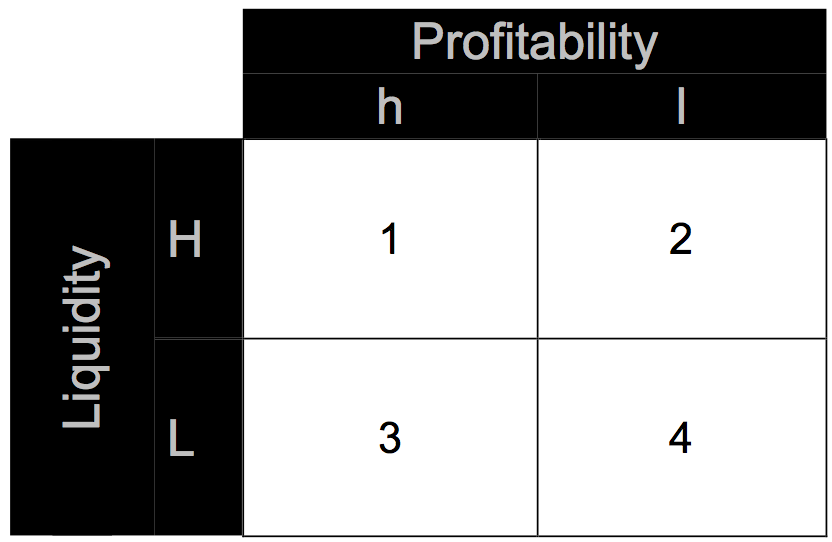
\includegraphics[width=9cm]{fig/plquadrant.jpg}}}
\caption[Liquidity--Profitability--Matrix]{Liquidity--Profitability--Matrix}
\captionsetup{font={footnotesize,it}}
\vspace{-0.3cm}
\caption*{Source: \cite[19]{Vieira:2010ve}}
\label{fig:plquadrant}
\end{figure}

\ni To cluster the companies he observed, \citeauthor{Vieira:2010ve} created a Liquidity--Profitability--Matrix (see
figure \vref{fig:plquadrant}).\endnote{\citeauthor{Vieira:2010ve} clustered the companies using the following rules:

\begin{itemize}
  \item Companies with liquidity ratio $> 1$ go in row \emph{H}, the others in row \emph{L}
  \item Companies with an average \gls{roa} for the observation period higher than the average
  market \gls{roa} went in row \emph{h}, the others in row \emph{l}.
\end{itemize}

\citeauthor{Vieira:2010ve} hypothesized the following behaviors (\citeyear[19]{Vieira:2010ve}):

\begin{itemize}
  \item Companies from quadrant 2 (Hl) would migrate to the quadrants 3 (lH) or 4 (Ll); and companies
  from quadrant 3 (Lh) would migrate to quadrants 2 (Hl) or 4 (Ll) \emph{because the low level of
  one of the indicators would deteriorate the other}.
  \item Companies from quadrants 1 (Hh) or 4 (Ll) would stay there \emph{as their extreme position---either
  good or bad---would lock them in and make it hard to change.}  
\end{itemize}}


\subsection{Results} \label{sec:results}

\subsubsection{Hypothesis 1: Short Term Negative Relationship between Liquidity and Profitability} \label{sec:res_h1}

Interestingly,  hypothesis  \vref{h1} was \emph{clearly rejected}: ``In fact it was
found a significant positive relationship between the indicators.''
(\citeyear[24]{Vieira:2010ve}) This result goes against the literature (see
sections \vref{sec:liquidity_profitability_trade_off} and
\vref{sec:risk_and_returns}), and \citeauthor{Vieira:2010ve} hypothesizes that
the studied industry sector (airlines) might differ significantly from other
sector.\endnote{As an example, this may be due to a high demand on current expenses (fuel, maintenance), hence a
high level of \gls{glos:workingcapital} (see section \vref{sec:cash_gap}) would
be directly related to reducing costs and obtaining higher profits; also, these
companies being rather large, they would be less likely to show a high demand on
liquidity compared to \glspl{glos:sme}---see also \citeauthor{Decman:2012vn} who
note that ``\Glspl{sme} are usually characterized by a high proportion of
current assets to total assets, less liquid, exposed to high volatility of cash
flows and mostly rely on short-term borrowing.'' (\citeyear[692]{Decman:2012vn}).}


\subsubsection{Hypothesis 2: Medium Term, low Liquidity will deteriorate Profitability, and vice versa} \label{sec:res_h2}

Hypothesis \vref{h2} was \emph{confirmed}, yet due to the rejection of hypothesis
\vref{h1}, ``lost part of its meaning:`` \citep[32]{Vieira:2010ve}: An inversion
was not observed, yet a dependency of the medium term relationship on the short
term results.

\subsubsection{Hypothesis 3: Over the year 2008, a higher liquidity helped achieve better performance} \label{sec:res_h3}



The performance indicators observed \emph{strongly confirmed} the hypothesis, as
companies with a higher liquidity had a comparatively better performance in
2008, reinforcing the view that ``the importance of the management of the
working capital increases during hard times.''
(\citeyear[31]{Vieira:2010ve})\endnote{Yet, as hypothesis \vref{h1} was
rejected, this ``lost its original sense, since it was expected that while the
relationship would be negative on the years of prosperity and then become
positive on the years of economic decline.'' (\citeyear[30]{Vieira:2010ve}) }



%</content>%



















% %=====================================================
% Chapter 4: Practical Experience
% 
% This is bringing in your experience in relation to the topic, either from 
% your work, or elsewhere. If you don't have any work experience in the 
% topic, you should ask your finance manager at work or CFO for any 
% ideas. If all fails then research on the Internet for relevant examples / 
% experience
%
% 20% of the word count (200 words)
%=====================================================

\def\hlIV{Practical Experience}\def\lbIV{sec:PracticalExperience}

\mnequals{\doctype}{book}{\chapter{\hlIV}}{\section{\hlIV}}\label{\lbIV}

%<content>%



%</content>%















































































% % ===================================================== 
% Chapter 5: Conclusions 
% A summary of the key points and a direct response to the question posed  
%
% 5% of the word count (50 words)
% =====================================================

\section{Conclusions} \label{sec:Conclusions}
% <content>%



% </content>%




















% %=====================================================
% Static Glossary etc. entries
%=====================================================
%
% Especially interesting if you have acronyms which are only introduced
% within the (later) glossary, hence would not have been used in the text,
% and hence would not appear in the list of acronyms. If you define them
% here, using \glslink{acronymname}{\null}, nothing will be output, yet
% the link will be established, hence the entry will be printed. Likewise,
% you can put here additional things you want to have in the list of acronyms
% (or glossary or symbols, for that matter) even if you do not reference them
% in the text (for whatever reason).
%
%=====================================================

%-----------------------------------------------------
% Samples
%-----------------------------------------------------

% Usage:
%
% \glslink{rosf}{\null}


%-----------------------------------------------------
% Content
%-----------------------------------------------------

%<content>%

\glslink{rosf}{\null}
\glslink{roce}{\null}



%</content>%
























% %=====================================================
% Chapter 99: Appendices
%=====================================================

%=====================================================
% Appendix
%=====================================================

\ifthenelse{\equal{\doctype}{book}}{
  \appendix
}{}

%=====================================================
% End Notes
%=====================================================

\phantomsection
\ifthenelse{\equal{\doctype}{book}}{
  \addcontentsline{toc}{chapter}{Notes}
}{
\addcontentsline{toc}{section}{Notes}
}
\pagestyle{fancy}
\fancyhead{}
\fancyhead[RE,RO]{\thepage}
\fancyhead[LE]{\slshape NOTES}
\fancyhead[LO]{\slshape NOTES}
\fancyfoot[C]{}
%\theendnotes \setcounter{endnote}{0}
\label{sec:notes}\printendnotes 
%\setcounter{endnote}{0}
%\clearpage{\pagestyle{empty}\cleardoublepage}
\clearpage




%=====================================================
% Acronyms and Symbols
%=====================================================

\phantomsection
\addcontentsline{toc}{section}{Acronyms and Symbols}
\pagestyle{fancy}
\fancyhead{}
\fancyhead[RE,RO]{\thepage}
\fancyhead[LE]{\slshape ACRONYMS AND SYMBOLS}
\fancyhead[LO]{\slshape ACRONYMS AND SYMBOLS}
\fancyfoot[C]{}
%\printacronym
%\printglossary[type=\acronymtype]
%Print list of acronyms
%\deftranslation[to=German]{Acronyms}{Abk�rzungsverzeichnis}
\label{sec:acronyms}\printglossary[type=\acronymtype,style=long]
%Print list of symbols
\label{sec:symbols}\printglossary[type=symbolslist,style=long]

%\clearpage{\pagestyle{empty}\cleardoublepage}
\clearpage


%=====================================================
% Glossary
%=====================================================

\phantomsection
\addcontentsline{toc}{section}{Glossary}
\pagestyle{fancy}
\fancyhead{}
\fancyhead[RE,RO]{\thepage}
\fancyhead[LE]{\slshape GLOSSARY}
\fancyhead[LO]{\slshape GLOSSARY}
\fancyfoot[C]{}
%\printglossary
%\printglossary[type=main]
\label{sec:glossary}\printglossary[style=altlist,title=Glossary]

%\clearpage{\pagestyle{empty}\cleardoublepage}
\clearpage


%=====================================================
% Index
%=====================================================

% Usage:
% \index{Fourier Series}

%
% Index comes with a plain page style, we hack it here so that we have
% the same pagestyle as everywhere else.
% 
\patchcmd{\theindex}% <cmd>
  {\thispagestyle{plain}}% <search>
  {\pagestyle{indexstyle}}% <replace>
  {}{}%
  \fancypagestyle{indexstyle}{%
\pagestyle{fancy}
\fancyhead{}
\fancyhead[RE,RO]{\thepage}
\fancyhead[LE]{\slshape INDEX}
\fancyhead[LO]{\slshape INDEX}
\fancyfoot[C]{}
 }
\renewcommand{\indexname}{Index}%

\phantomsection
\addcontentsline{toc}{section}{Index}
\label{sec:index}\printindex
%\clearpage{\pagestyle{empty}\cleardoublepage}
\clearpage


%=====================================================
% References
%=====================================================
\phantomsection
\addcontentsline{toc}{section}{References}
\pagestyle{fancy}
\fancyhead{}
\fancyhead[RE,RO]{\thepage}
\fancyhead[LE]{\slshape REFERENCES}
\fancyhead[LO]{\slshape REFERENCES}
\fancyfoot[C]{}
%\begin{thebibliography}{99}
\patchcmd{\bibsetup}{\interlinepenalty=5000}{\interlinepenalty=10000}{}{}
\label{sec:bibliography}\printbibliography
%\end{thebibliography}
%\clearpage{\pagestyle{empty}\cleardoublepage}
%\clearpage


 










































  \wcounta
  %=====================================================
% Chapter 1: Introduction
% 
% This is not a re-hash of the question but an introduction to your submission
%
% 5% of the word count (50 words)
%=====================================================
% Chapter 1:  5 %  Introduction
% Chapter 2: 30 % Literature Review
% Chapter 3: 40 % Application of the Literature to the Question
% Chapter 4: 20 % Practical Experience
% Chapter 5: 10 % Conclusions
%=====================================================

\section{Introduction}\label{sec:Introduction}
% <content>%



%</content>%






















  %=====================================================
% Chapter 2: Literature Review
% 
% Summary of the relevant articles you have located in the library that can 
% be used to help you address the question.
%
% 30% of the word count (300 words)
%=====================================================

\def\hlII{Literature Review}\def\lbII{sec:LiteratureReview}

\mnequals{\doctype}{book}{\chapter{\hlII}}{\section{\hlII}}\label{\lbII}

%<content>%



%</content>%













































































  %=====================================================
% Chapter 3: Application of the Literature to the Question
% 
% You use the literature that you have found, together with your own views 
% to formulate your answer
%
% 40% of the word count (400 words)
%=====================================================

\section{Application} \label{sec:Application}
% <content>%

\subsection{Case Study} \label{sec:case_study}

\citeauthor{Vieira:2010ve} applied the findings to the airline industry in the context
of the Lehman crisis (2008) to verify three hypotheses (\citeyear[15]{Vieira:2010ve}):

\begin{enumerate}
  \item \emph{Hypothesis:} ``On the short term  the relationship between liquidity and profitability is negative.'' \label{h1}
  \item \emph{Hypothesis:} ``On the medium term a low liquidity level will derail the upkeep of high 
  profitability, and also a low profitability will derail the upkeep of a high liquidity.'' \label{h2}
  \item \emph{Hypothesis:}``Over the year of 2008, the companies with higher liquidity would be able to
  achieve a better performance.''  \label{h3}
\end{enumerate}

\begin{figure}[htp]
\centerline{\framebox{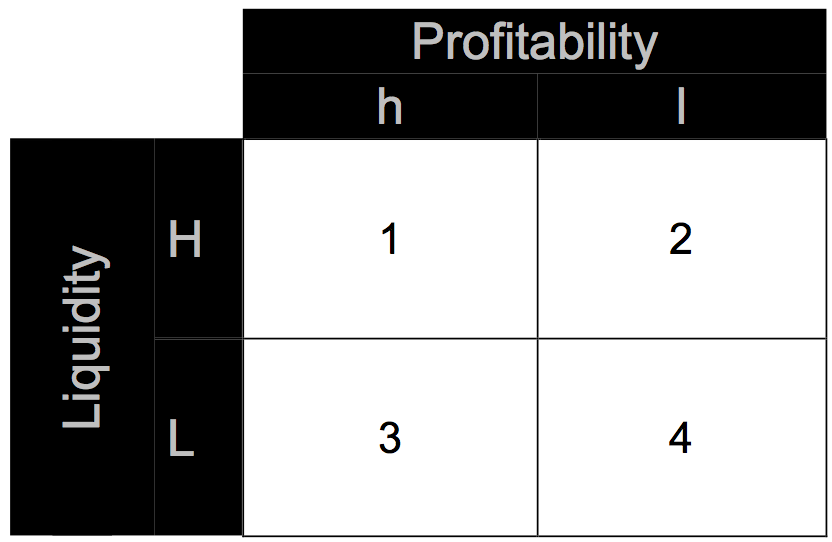
\includegraphics[width=9cm]{fig/plquadrant.jpg}}}
\caption[Liquidity--Profitability--Matrix]{Liquidity--Profitability--Matrix}
\captionsetup{font={footnotesize,it}}
\vspace{-0.3cm}
\caption*{Source: \cite[19]{Vieira:2010ve}}
\label{fig:plquadrant}
\end{figure}

\ni To cluster the companies he observed, \citeauthor{Vieira:2010ve} created a Liquidity--Profitability--Matrix (see
figure \vref{fig:plquadrant}).\endnote{\citeauthor{Vieira:2010ve} clustered the companies using the following rules:

\begin{itemize}
  \item Companies with liquidity ratio $> 1$ go in row \emph{H}, the others in row \emph{L}
  \item Companies with an average \gls{roa} for the observation period higher than the average
  market \gls{roa} went in row \emph{h}, the others in row \emph{l}.
\end{itemize}

\citeauthor{Vieira:2010ve} hypothesized the following behaviors (\citeyear[19]{Vieira:2010ve}):

\begin{itemize}
  \item Companies from quadrant 2 (Hl) would migrate to the quadrants 3 (lH) or 4 (Ll); and companies
  from quadrant 3 (Lh) would migrate to quadrants 2 (Hl) or 4 (Ll) \emph{because the low level of
  one of the indicators would deteriorate the other}.
  \item Companies from quadrants 1 (Hh) or 4 (Ll) would stay there \emph{as their extreme position---either
  good or bad---would lock them in and make it hard to change.}  
\end{itemize}}


\subsection{Results} \label{sec:results}

\subsubsection{Hypothesis 1: Short Term Negative Relationship between Liquidity and Profitability} \label{sec:res_h1}

Interestingly,  hypothesis  \vref{h1} was \emph{clearly rejected}: ``In fact it was
found a significant positive relationship between the indicators.''
(\citeyear[24]{Vieira:2010ve}) This result goes against the literature (see
sections \vref{sec:liquidity_profitability_trade_off} and
\vref{sec:risk_and_returns}), and \citeauthor{Vieira:2010ve} hypothesizes that
the studied industry sector (airlines) might differ significantly from other
sector.\endnote{As an example, this may be due to a high demand on current expenses (fuel, maintenance), hence a
high level of \gls{glos:workingcapital} (see section \vref{sec:cash_gap}) would
be directly related to reducing costs and obtaining higher profits; also, these
companies being rather large, they would be less likely to show a high demand on
liquidity compared to \glspl{glos:sme}---see also \citeauthor{Decman:2012vn} who
note that ``\Glspl{sme} are usually characterized by a high proportion of
current assets to total assets, less liquid, exposed to high volatility of cash
flows and mostly rely on short-term borrowing.'' (\citeyear[692]{Decman:2012vn}).}


\subsubsection{Hypothesis 2: Medium Term, low Liquidity will deteriorate Profitability, and vice versa} \label{sec:res_h2}

Hypothesis \vref{h2} was \emph{confirmed}, yet due to the rejection of hypothesis
\vref{h1}, ``lost part of its meaning:`` \citep[32]{Vieira:2010ve}: An inversion
was not observed, yet a dependency of the medium term relationship on the short
term results.

\subsubsection{Hypothesis 3: Over the year 2008, a higher liquidity helped achieve better performance} \label{sec:res_h3}



The performance indicators observed \emph{strongly confirmed} the hypothesis, as
companies with a higher liquidity had a comparatively better performance in
2008, reinforcing the view that ``the importance of the management of the
working capital increases during hard times.''
(\citeyear[31]{Vieira:2010ve})\endnote{Yet, as hypothesis \vref{h1} was
rejected, this ``lost its original sense, since it was expected that while the
relationship would be negative on the years of prosperity and then become
positive on the years of economic decline.'' (\citeyear[30]{Vieira:2010ve}) }



%</content>%



















  %=====================================================
% Chapter 4: Practical Experience
% 
% This is bringing in your experience in relation to the topic, either from 
% your work, or elsewhere. If you don't have any work experience in the 
% topic, you should ask your finance manager at work or CFO for any 
% ideas. If all fails then research on the Internet for relevant examples / 
% experience
%
% 20% of the word count (200 words)
%=====================================================

\def\hlIV{Practical Experience}\def\lbIV{sec:PracticalExperience}

\mnequals{\doctype}{book}{\chapter{\hlIV}}{\section{\hlIV}}\label{\lbIV}

%<content>%



%</content>%















































































  % ===================================================== 
% Chapter 5: Conclusions 
% A summary of the key points and a direct response to the question posed  
%
% 5% of the word count (50 words)
% =====================================================

\section{Conclusions} \label{sec:Conclusions}
% <content>%



% </content>%




















  \wcounte 
  }{
  % ===================================================== 
% Chapter 0: Topic
% =====================================================

\pagestyle{fancy}
\fancyhead{}
\fancyhead[RE,RO]{\thepage} \fancyhead[LE]{\slshape \leftmark}
\fancyhead[LO]{\slshape \leftmark}
\fancyfoot{\companyfooter}

%\renewcommand\submit{true}
\wcounte
\mnequals{\submit}{true}{}{
\mnequals{\doctype}{book}{
\chapter*{Notes}
}{
\section*{Notes}
% <content>%



%</content>% 

\section*{Discussion Question Answer}}}
\wcounta

%=====================================================
% Include Content and Appendices
%=====================================================

% %=====================================================
% Chapter 1: Introduction
% 
% This is not a re-hash of the question but an introduction to your submission
%
% 5% of the word count (50 words)
%=====================================================
% Chapter 1:  5 %  Introduction
% Chapter 2: 30 % Literature Review
% Chapter 3: 40 % Application of the Literature to the Question
% Chapter 4: 20 % Practical Experience
% Chapter 5: 10 % Conclusions
%=====================================================

\section{Introduction}\label{sec:Introduction}
% <content>%



%</content>%






















% %=====================================================
% Chapter 2: Literature Review
% 
% Summary of the relevant articles you have located in the library that can 
% be used to help you address the question.
%
% 30% of the word count (300 words)
%=====================================================

\def\hlII{Literature Review}\def\lbII{sec:LiteratureReview}

\mnequals{\doctype}{book}{\chapter{\hlII}}{\section{\hlII}}\label{\lbII}

%<content>%



%</content>%













































































% %=====================================================
% Chapter 3: Application of the Literature to the Question
% 
% You use the literature that you have found, together with your own views 
% to formulate your answer
%
% 40% of the word count (400 words)
%=====================================================

\section{Application} \label{sec:Application}
% <content>%

\subsection{Case Study} \label{sec:case_study}

\citeauthor{Vieira:2010ve} applied the findings to the airline industry in the context
of the Lehman crisis (2008) to verify three hypotheses (\citeyear[15]{Vieira:2010ve}):

\begin{enumerate}
  \item \emph{Hypothesis:} ``On the short term  the relationship between liquidity and profitability is negative.'' \label{h1}
  \item \emph{Hypothesis:} ``On the medium term a low liquidity level will derail the upkeep of high 
  profitability, and also a low profitability will derail the upkeep of a high liquidity.'' \label{h2}
  \item \emph{Hypothesis:}``Over the year of 2008, the companies with higher liquidity would be able to
  achieve a better performance.''  \label{h3}
\end{enumerate}

\begin{figure}[htp]
\centerline{\framebox{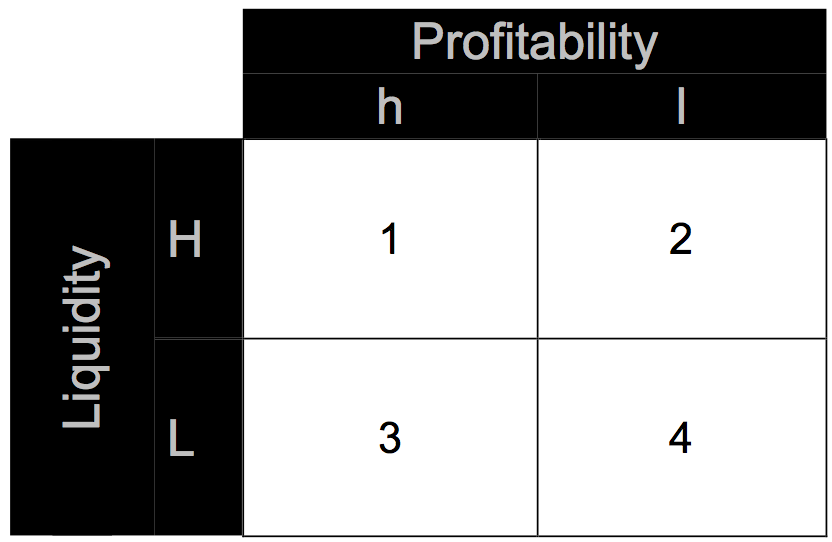
\includegraphics[width=9cm]{fig/plquadrant.jpg}}}
\caption[Liquidity--Profitability--Matrix]{Liquidity--Profitability--Matrix}
\captionsetup{font={footnotesize,it}}
\vspace{-0.3cm}
\caption*{Source: \cite[19]{Vieira:2010ve}}
\label{fig:plquadrant}
\end{figure}

\ni To cluster the companies he observed, \citeauthor{Vieira:2010ve} created a Liquidity--Profitability--Matrix (see
figure \vref{fig:plquadrant}).\endnote{\citeauthor{Vieira:2010ve} clustered the companies using the following rules:

\begin{itemize}
  \item Companies with liquidity ratio $> 1$ go in row \emph{H}, the others in row \emph{L}
  \item Companies with an average \gls{roa} for the observation period higher than the average
  market \gls{roa} went in row \emph{h}, the others in row \emph{l}.
\end{itemize}

\citeauthor{Vieira:2010ve} hypothesized the following behaviors (\citeyear[19]{Vieira:2010ve}):

\begin{itemize}
  \item Companies from quadrant 2 (Hl) would migrate to the quadrants 3 (lH) or 4 (Ll); and companies
  from quadrant 3 (Lh) would migrate to quadrants 2 (Hl) or 4 (Ll) \emph{because the low level of
  one of the indicators would deteriorate the other}.
  \item Companies from quadrants 1 (Hh) or 4 (Ll) would stay there \emph{as their extreme position---either
  good or bad---would lock them in and make it hard to change.}  
\end{itemize}}


\subsection{Results} \label{sec:results}

\subsubsection{Hypothesis 1: Short Term Negative Relationship between Liquidity and Profitability} \label{sec:res_h1}

Interestingly,  hypothesis  \vref{h1} was \emph{clearly rejected}: ``In fact it was
found a significant positive relationship between the indicators.''
(\citeyear[24]{Vieira:2010ve}) This result goes against the literature (see
sections \vref{sec:liquidity_profitability_trade_off} and
\vref{sec:risk_and_returns}), and \citeauthor{Vieira:2010ve} hypothesizes that
the studied industry sector (airlines) might differ significantly from other
sector.\endnote{As an example, this may be due to a high demand on current expenses (fuel, maintenance), hence a
high level of \gls{glos:workingcapital} (see section \vref{sec:cash_gap}) would
be directly related to reducing costs and obtaining higher profits; also, these
companies being rather large, they would be less likely to show a high demand on
liquidity compared to \glspl{glos:sme}---see also \citeauthor{Decman:2012vn} who
note that ``\Glspl{sme} are usually characterized by a high proportion of
current assets to total assets, less liquid, exposed to high volatility of cash
flows and mostly rely on short-term borrowing.'' (\citeyear[692]{Decman:2012vn}).}


\subsubsection{Hypothesis 2: Medium Term, low Liquidity will deteriorate Profitability, and vice versa} \label{sec:res_h2}

Hypothesis \vref{h2} was \emph{confirmed}, yet due to the rejection of hypothesis
\vref{h1}, ``lost part of its meaning:`` \citep[32]{Vieira:2010ve}: An inversion
was not observed, yet a dependency of the medium term relationship on the short
term results.

\subsubsection{Hypothesis 3: Over the year 2008, a higher liquidity helped achieve better performance} \label{sec:res_h3}



The performance indicators observed \emph{strongly confirmed} the hypothesis, as
companies with a higher liquidity had a comparatively better performance in
2008, reinforcing the view that ``the importance of the management of the
working capital increases during hard times.''
(\citeyear[31]{Vieira:2010ve})\endnote{Yet, as hypothesis \vref{h1} was
rejected, this ``lost its original sense, since it was expected that while the
relationship would be negative on the years of prosperity and then become
positive on the years of economic decline.'' (\citeyear[30]{Vieira:2010ve}) }



%</content>%



















% %=====================================================
% Chapter 4: Practical Experience
% 
% This is bringing in your experience in relation to the topic, either from 
% your work, or elsewhere. If you don't have any work experience in the 
% topic, you should ask your finance manager at work or CFO for any 
% ideas. If all fails then research on the Internet for relevant examples / 
% experience
%
% 20% of the word count (200 words)
%=====================================================

\def\hlIV{Practical Experience}\def\lbIV{sec:PracticalExperience}

\mnequals{\doctype}{book}{\chapter{\hlIV}}{\section{\hlIV}}\label{\lbIV}

%<content>%



%</content>%















































































% % ===================================================== 
% Chapter 5: Conclusions 
% A summary of the key points and a direct response to the question posed  
%
% 5% of the word count (50 words)
% =====================================================

\section{Conclusions} \label{sec:Conclusions}
% <content>%



% </content>%




















% %=====================================================
% Static Glossary etc. entries
%=====================================================
%
% Especially interesting if you have acronyms which are only introduced
% within the (later) glossary, hence would not have been used in the text,
% and hence would not appear in the list of acronyms. If you define them
% here, using \glslink{acronymname}{\null}, nothing will be output, yet
% the link will be established, hence the entry will be printed. Likewise,
% you can put here additional things you want to have in the list of acronyms
% (or glossary or symbols, for that matter) even if you do not reference them
% in the text (for whatever reason).
%
%=====================================================

%-----------------------------------------------------
% Samples
%-----------------------------------------------------

% Usage:
%
% \glslink{rosf}{\null}


%-----------------------------------------------------
% Content
%-----------------------------------------------------

%<content>%

\glslink{rosf}{\null}
\glslink{roce}{\null}



%</content>%
























% %=====================================================
% Chapter 99: Appendices
%=====================================================

%=====================================================
% Appendix
%=====================================================

\ifthenelse{\equal{\doctype}{book}}{
  \appendix
}{}

%=====================================================
% End Notes
%=====================================================

\phantomsection
\ifthenelse{\equal{\doctype}{book}}{
  \addcontentsline{toc}{chapter}{Notes}
}{
\addcontentsline{toc}{section}{Notes}
}
\pagestyle{fancy}
\fancyhead{}
\fancyhead[RE,RO]{\thepage}
\fancyhead[LE]{\slshape NOTES}
\fancyhead[LO]{\slshape NOTES}
\fancyfoot[C]{}
%\theendnotes \setcounter{endnote}{0}
\label{sec:notes}\printendnotes 
%\setcounter{endnote}{0}
%\clearpage{\pagestyle{empty}\cleardoublepage}
\clearpage




%=====================================================
% Acronyms and Symbols
%=====================================================

\phantomsection
\addcontentsline{toc}{section}{Acronyms and Symbols}
\pagestyle{fancy}
\fancyhead{}
\fancyhead[RE,RO]{\thepage}
\fancyhead[LE]{\slshape ACRONYMS AND SYMBOLS}
\fancyhead[LO]{\slshape ACRONYMS AND SYMBOLS}
\fancyfoot[C]{}
%\printacronym
%\printglossary[type=\acronymtype]
%Print list of acronyms
%\deftranslation[to=German]{Acronyms}{Abk�rzungsverzeichnis}
\label{sec:acronyms}\printglossary[type=\acronymtype,style=long]
%Print list of symbols
\label{sec:symbols}\printglossary[type=symbolslist,style=long]

%\clearpage{\pagestyle{empty}\cleardoublepage}
\clearpage


%=====================================================
% Glossary
%=====================================================

\phantomsection
\addcontentsline{toc}{section}{Glossary}
\pagestyle{fancy}
\fancyhead{}
\fancyhead[RE,RO]{\thepage}
\fancyhead[LE]{\slshape GLOSSARY}
\fancyhead[LO]{\slshape GLOSSARY}
\fancyfoot[C]{}
%\printglossary
%\printglossary[type=main]
\label{sec:glossary}\printglossary[style=altlist,title=Glossary]

%\clearpage{\pagestyle{empty}\cleardoublepage}
\clearpage


%=====================================================
% Index
%=====================================================

% Usage:
% \index{Fourier Series}

%
% Index comes with a plain page style, we hack it here so that we have
% the same pagestyle as everywhere else.
% 
\patchcmd{\theindex}% <cmd>
  {\thispagestyle{plain}}% <search>
  {\pagestyle{indexstyle}}% <replace>
  {}{}%
  \fancypagestyle{indexstyle}{%
\pagestyle{fancy}
\fancyhead{}
\fancyhead[RE,RO]{\thepage}
\fancyhead[LE]{\slshape INDEX}
\fancyhead[LO]{\slshape INDEX}
\fancyfoot[C]{}
 }
\renewcommand{\indexname}{Index}%

\phantomsection
\addcontentsline{toc}{section}{Index}
\label{sec:index}\printindex
%\clearpage{\pagestyle{empty}\cleardoublepage}
\clearpage


%=====================================================
% References
%=====================================================
\phantomsection
\addcontentsline{toc}{section}{References}
\pagestyle{fancy}
\fancyhead{}
\fancyhead[RE,RO]{\thepage}
\fancyhead[LE]{\slshape REFERENCES}
\fancyhead[LO]{\slshape REFERENCES}
\fancyfoot[C]{}
%\begin{thebibliography}{99}
\patchcmd{\bibsetup}{\interlinepenalty=5000}{\interlinepenalty=10000}{}{}
\label{sec:bibliography}\printbibliography
%\end{thebibliography}
%\clearpage{\pagestyle{empty}\cleardoublepage}
%\clearpage


 









































 
  \wcounta 
  %=====================================================
% Chapter 1: Introduction
% 
% This is not a re-hash of the question but an introduction to your submission
%
% 5% of the word count (50 words)
%=====================================================
% Chapter 1:  5 %  Introduction
% Chapter 2: 30 % Literature Review
% Chapter 3: 40 % Application of the Literature to the Question
% Chapter 4: 20 % Practical Experience
% Chapter 5: 10 % Conclusions
%=====================================================

\section{Introduction}\label{sec:Introduction}
% <content>%



%</content>%






















  %=====================================================
% Chapter 2: Literature Review
% 
% Summary of the relevant articles you have located in the library that can 
% be used to help you address the question.
%
% 30% of the word count (300 words)
%=====================================================

\def\hlII{Literature Review}\def\lbII{sec:LiteratureReview}

\mnequals{\doctype}{book}{\chapter{\hlII}}{\section{\hlII}}\label{\lbII}

%<content>%



%</content>%













































































  %=====================================================
% Chapter 3: Application of the Literature to the Question
% 
% You use the literature that you have found, together with your own views 
% to formulate your answer
%
% 40% of the word count (400 words)
%=====================================================

\section{Application} \label{sec:Application}
% <content>%

\subsection{Case Study} \label{sec:case_study}

\citeauthor{Vieira:2010ve} applied the findings to the airline industry in the context
of the Lehman crisis (2008) to verify three hypotheses (\citeyear[15]{Vieira:2010ve}):

\begin{enumerate}
  \item \emph{Hypothesis:} ``On the short term  the relationship between liquidity and profitability is negative.'' \label{h1}
  \item \emph{Hypothesis:} ``On the medium term a low liquidity level will derail the upkeep of high 
  profitability, and also a low profitability will derail the upkeep of a high liquidity.'' \label{h2}
  \item \emph{Hypothesis:}``Over the year of 2008, the companies with higher liquidity would be able to
  achieve a better performance.''  \label{h3}
\end{enumerate}

\begin{figure}[htp]
\centerline{\framebox{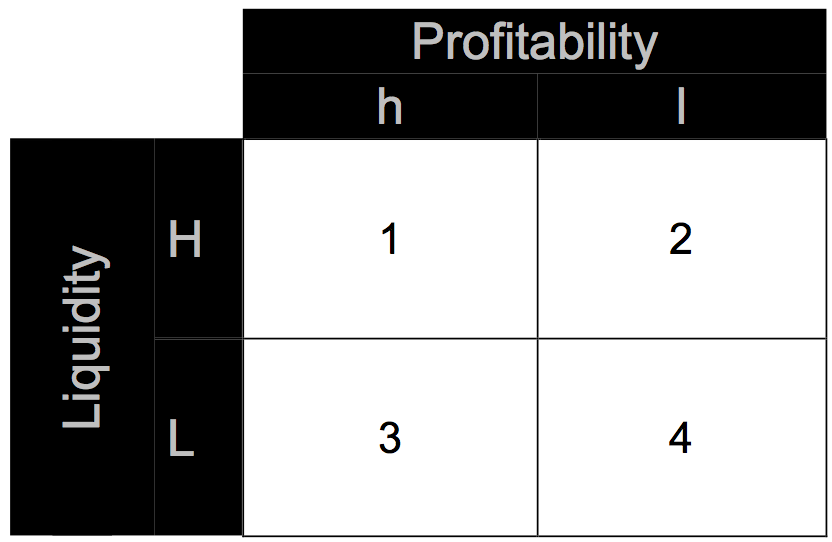
\includegraphics[width=9cm]{fig/plquadrant.jpg}}}
\caption[Liquidity--Profitability--Matrix]{Liquidity--Profitability--Matrix}
\captionsetup{font={footnotesize,it}}
\vspace{-0.3cm}
\caption*{Source: \cite[19]{Vieira:2010ve}}
\label{fig:plquadrant}
\end{figure}

\ni To cluster the companies he observed, \citeauthor{Vieira:2010ve} created a Liquidity--Profitability--Matrix (see
figure \vref{fig:plquadrant}).\endnote{\citeauthor{Vieira:2010ve} clustered the companies using the following rules:

\begin{itemize}
  \item Companies with liquidity ratio $> 1$ go in row \emph{H}, the others in row \emph{L}
  \item Companies with an average \gls{roa} for the observation period higher than the average
  market \gls{roa} went in row \emph{h}, the others in row \emph{l}.
\end{itemize}

\citeauthor{Vieira:2010ve} hypothesized the following behaviors (\citeyear[19]{Vieira:2010ve}):

\begin{itemize}
  \item Companies from quadrant 2 (Hl) would migrate to the quadrants 3 (lH) or 4 (Ll); and companies
  from quadrant 3 (Lh) would migrate to quadrants 2 (Hl) or 4 (Ll) \emph{because the low level of
  one of the indicators would deteriorate the other}.
  \item Companies from quadrants 1 (Hh) or 4 (Ll) would stay there \emph{as their extreme position---either
  good or bad---would lock them in and make it hard to change.}  
\end{itemize}}


\subsection{Results} \label{sec:results}

\subsubsection{Hypothesis 1: Short Term Negative Relationship between Liquidity and Profitability} \label{sec:res_h1}

Interestingly,  hypothesis  \vref{h1} was \emph{clearly rejected}: ``In fact it was
found a significant positive relationship between the indicators.''
(\citeyear[24]{Vieira:2010ve}) This result goes against the literature (see
sections \vref{sec:liquidity_profitability_trade_off} and
\vref{sec:risk_and_returns}), and \citeauthor{Vieira:2010ve} hypothesizes that
the studied industry sector (airlines) might differ significantly from other
sector.\endnote{As an example, this may be due to a high demand on current expenses (fuel, maintenance), hence a
high level of \gls{glos:workingcapital} (see section \vref{sec:cash_gap}) would
be directly related to reducing costs and obtaining higher profits; also, these
companies being rather large, they would be less likely to show a high demand on
liquidity compared to \glspl{glos:sme}---see also \citeauthor{Decman:2012vn} who
note that ``\Glspl{sme} are usually characterized by a high proportion of
current assets to total assets, less liquid, exposed to high volatility of cash
flows and mostly rely on short-term borrowing.'' (\citeyear[692]{Decman:2012vn}).}


\subsubsection{Hypothesis 2: Medium Term, low Liquidity will deteriorate Profitability, and vice versa} \label{sec:res_h2}

Hypothesis \vref{h2} was \emph{confirmed}, yet due to the rejection of hypothesis
\vref{h1}, ``lost part of its meaning:`` \citep[32]{Vieira:2010ve}: An inversion
was not observed, yet a dependency of the medium term relationship on the short
term results.

\subsubsection{Hypothesis 3: Over the year 2008, a higher liquidity helped achieve better performance} \label{sec:res_h3}



The performance indicators observed \emph{strongly confirmed} the hypothesis, as
companies with a higher liquidity had a comparatively better performance in
2008, reinforcing the view that ``the importance of the management of the
working capital increases during hard times.''
(\citeyear[31]{Vieira:2010ve})\endnote{Yet, as hypothesis \vref{h1} was
rejected, this ``lost its original sense, since it was expected that while the
relationship would be negative on the years of prosperity and then become
positive on the years of economic decline.'' (\citeyear[30]{Vieira:2010ve}) }



%</content>%



















  %=====================================================
% Chapter 4: Practical Experience
% 
% This is bringing in your experience in relation to the topic, either from 
% your work, or elsewhere. If you don't have any work experience in the 
% topic, you should ask your finance manager at work or CFO for any 
% ideas. If all fails then research on the Internet for relevant examples / 
% experience
%
% 20% of the word count (200 words)
%=====================================================

\def\hlIV{Practical Experience}\def\lbIV{sec:PracticalExperience}

\mnequals{\doctype}{book}{\chapter{\hlIV}}{\section{\hlIV}}\label{\lbIV}

%<content>%



%</content>%















































































  % ===================================================== 
% Chapter 5: Conclusions 
% A summary of the key points and a direct response to the question posed  
%
% 5% of the word count (50 words)
% =====================================================

\section{Conclusions} \label{sec:Conclusions}
% <content>%



% </content>%




















  \wcounte 
}

%=====================================================
% Word Count
%=====================================================

%\bigskip \hfill \emph{\input{tmp/wc.tex}}\emph{Words} excluding front matter, exhibits, %notes and appendices.\bigskip


%=====================================================
% Include Appendices
%=====================================================

%=====================================================
% Static Glossary etc. entries
%=====================================================
%
% Especially interesting if you have acronyms which are only introduced
% within the (later) glossary, hence would not have been used in the text,
% and hence would not appear in the list of acronyms. If you define them
% here, using \glslink{acronymname}{\null}, nothing will be output, yet
% the link will be established, hence the entry will be printed. Likewise,
% you can put here additional things you want to have in the list of acronyms
% (or glossary or symbols, for that matter) even if you do not reference them
% in the text (for whatever reason).
%
%=====================================================

%-----------------------------------------------------
% Samples
%-----------------------------------------------------

% Usage:
%
% \glslink{rosf}{\null}


%-----------------------------------------------------
% Content
%-----------------------------------------------------

%<content>%

\glslink{rosf}{\null}
\glslink{roce}{\null}



%</content>%

























\makeatletter
\ifthenelse{\equal{\doctype}{book}}{
\@openrightfalse
\part{Appendix}


 \appendix
 %=====================================================
% Chapter 99: Appendices
%=====================================================

%=====================================================
% Appendix
%=====================================================

\ifthenelse{\equal{\doctype}{book}}{
  \appendix
}{}

%=====================================================
% End Notes
%=====================================================

\phantomsection
\ifthenelse{\equal{\doctype}{book}}{
  \addcontentsline{toc}{chapter}{Notes}
}{
\addcontentsline{toc}{section}{Notes}
}
\pagestyle{fancy}
\fancyhead{}
\fancyhead[RE,RO]{\thepage}
\fancyhead[LE]{\slshape NOTES}
\fancyhead[LO]{\slshape NOTES}
\fancyfoot[C]{}
%\theendnotes \setcounter{endnote}{0}
\label{sec:notes}\printendnotes 
%\setcounter{endnote}{0}
%\clearpage{\pagestyle{empty}\cleardoublepage}
\clearpage




%=====================================================
% Acronyms and Symbols
%=====================================================

\phantomsection
\addcontentsline{toc}{section}{Acronyms and Symbols}
\pagestyle{fancy}
\fancyhead{}
\fancyhead[RE,RO]{\thepage}
\fancyhead[LE]{\slshape ACRONYMS AND SYMBOLS}
\fancyhead[LO]{\slshape ACRONYMS AND SYMBOLS}
\fancyfoot[C]{}
%\printacronym
%\printglossary[type=\acronymtype]
%Print list of acronyms
%\deftranslation[to=German]{Acronyms}{Abk�rzungsverzeichnis}
\label{sec:acronyms}\printglossary[type=\acronymtype,style=long]
%Print list of symbols
\label{sec:symbols}\printglossary[type=symbolslist,style=long]

%\clearpage{\pagestyle{empty}\cleardoublepage}
\clearpage


%=====================================================
% Glossary
%=====================================================

\phantomsection
\addcontentsline{toc}{section}{Glossary}
\pagestyle{fancy}
\fancyhead{}
\fancyhead[RE,RO]{\thepage}
\fancyhead[LE]{\slshape GLOSSARY}
\fancyhead[LO]{\slshape GLOSSARY}
\fancyfoot[C]{}
%\printglossary
%\printglossary[type=main]
\label{sec:glossary}\printglossary[style=altlist,title=Glossary]

%\clearpage{\pagestyle{empty}\cleardoublepage}
\clearpage


%=====================================================
% Index
%=====================================================

% Usage:
% \index{Fourier Series}

%
% Index comes with a plain page style, we hack it here so that we have
% the same pagestyle as everywhere else.
% 
\patchcmd{\theindex}% <cmd>
  {\thispagestyle{plain}}% <search>
  {\pagestyle{indexstyle}}% <replace>
  {}{}%
  \fancypagestyle{indexstyle}{%
\pagestyle{fancy}
\fancyhead{}
\fancyhead[RE,RO]{\thepage}
\fancyhead[LE]{\slshape INDEX}
\fancyhead[LO]{\slshape INDEX}
\fancyfoot[C]{}
 }
\renewcommand{\indexname}{Index}%

\phantomsection
\addcontentsline{toc}{section}{Index}
\label{sec:index}\printindex
%\clearpage{\pagestyle{empty}\cleardoublepage}
\clearpage


%=====================================================
% References
%=====================================================
\phantomsection
\addcontentsline{toc}{section}{References}
\pagestyle{fancy}
\fancyhead{}
\fancyhead[RE,RO]{\thepage}
\fancyhead[LE]{\slshape REFERENCES}
\fancyhead[LO]{\slshape REFERENCES}
\fancyfoot[C]{}
%\begin{thebibliography}{99}
\patchcmd{\bibsetup}{\interlinepenalty=5000}{\interlinepenalty=10000}{}{}
\label{sec:bibliography}\printbibliography
%\end{thebibliography}
%\clearpage{\pagestyle{empty}\cleardoublepage}
%\clearpage


 

\@openrighttrue
\batchmode
}{
%=====================================================
% Chapter 99: Appendices
%=====================================================

%=====================================================
% Appendix
%=====================================================

\ifthenelse{\equal{\doctype}{book}}{
  \appendix
}{}

%=====================================================
% End Notes
%=====================================================

\phantomsection
\ifthenelse{\equal{\doctype}{book}}{
  \addcontentsline{toc}{chapter}{Notes}
}{
\addcontentsline{toc}{section}{Notes}
}
\pagestyle{fancy}
\fancyhead{}
\fancyhead[RE,RO]{\thepage}
\fancyhead[LE]{\slshape NOTES}
\fancyhead[LO]{\slshape NOTES}
\fancyfoot[C]{}
%\theendnotes \setcounter{endnote}{0}
\label{sec:notes}\printendnotes 
%\setcounter{endnote}{0}
%\clearpage{\pagestyle{empty}\cleardoublepage}
\clearpage




%=====================================================
% Acronyms and Symbols
%=====================================================

\phantomsection
\addcontentsline{toc}{section}{Acronyms and Symbols}
\pagestyle{fancy}
\fancyhead{}
\fancyhead[RE,RO]{\thepage}
\fancyhead[LE]{\slshape ACRONYMS AND SYMBOLS}
\fancyhead[LO]{\slshape ACRONYMS AND SYMBOLS}
\fancyfoot[C]{}
%\printacronym
%\printglossary[type=\acronymtype]
%Print list of acronyms
%\deftranslation[to=German]{Acronyms}{Abk�rzungsverzeichnis}
\label{sec:acronyms}\printglossary[type=\acronymtype,style=long]
%Print list of symbols
\label{sec:symbols}\printglossary[type=symbolslist,style=long]

%\clearpage{\pagestyle{empty}\cleardoublepage}
\clearpage


%=====================================================
% Glossary
%=====================================================

\phantomsection
\addcontentsline{toc}{section}{Glossary}
\pagestyle{fancy}
\fancyhead{}
\fancyhead[RE,RO]{\thepage}
\fancyhead[LE]{\slshape GLOSSARY}
\fancyhead[LO]{\slshape GLOSSARY}
\fancyfoot[C]{}
%\printglossary
%\printglossary[type=main]
\label{sec:glossary}\printglossary[style=altlist,title=Glossary]

%\clearpage{\pagestyle{empty}\cleardoublepage}
\clearpage


%=====================================================
% Index
%=====================================================

% Usage:
% \index{Fourier Series}

%
% Index comes with a plain page style, we hack it here so that we have
% the same pagestyle as everywhere else.
% 
\patchcmd{\theindex}% <cmd>
  {\thispagestyle{plain}}% <search>
  {\pagestyle{indexstyle}}% <replace>
  {}{}%
  \fancypagestyle{indexstyle}{%
\pagestyle{fancy}
\fancyhead{}
\fancyhead[RE,RO]{\thepage}
\fancyhead[LE]{\slshape INDEX}
\fancyhead[LO]{\slshape INDEX}
\fancyfoot[C]{}
 }
\renewcommand{\indexname}{Index}%

\phantomsection
\addcontentsline{toc}{section}{Index}
\label{sec:index}\printindex
%\clearpage{\pagestyle{empty}\cleardoublepage}
\clearpage


%=====================================================
% References
%=====================================================
\phantomsection
\addcontentsline{toc}{section}{References}
\pagestyle{fancy}
\fancyhead{}
\fancyhead[RE,RO]{\thepage}
\fancyhead[LE]{\slshape REFERENCES}
\fancyhead[LO]{\slshape REFERENCES}
\fancyfoot[C]{}
%\begin{thebibliography}{99}
\patchcmd{\bibsetup}{\interlinepenalty=5000}{\interlinepenalty=10000}{}{}
\label{sec:bibliography}\printbibliography
%\end{thebibliography}
%\clearpage{\pagestyle{empty}\cleardoublepage}
%\clearpage


 
}
\makeatother


%=====================================================
% End Document.
%=====================================================

\end{document}
